%---------------------------------------------------------------------
% Course 	: Introduction To web sciences
% Professor : Dr.Nelson
% Name   	: Manoj Chandra Kompalli
% Assignment: 10
%---------------------------------------------------------------------
\documentclass[12pt]{article}
%--------------------------------------------------------------------
% packages required
%--------------------------------------------------------------------
\usepackage{graphicx}
\usepackage{listings}
\usepackage{hyperref}
\usepackage{caption}
\usepackage{color}
\usepackage{pdfpages}
\graphicspath{ {images/} }
%--------------------------------------------------------------------
% Start Margins
%--------------------------------------------------------------------
\addtolength{\oddsidemargin}{-.875in}
\addtolength{\evensidemargin}{-.875in}
\addtolength{\textwidth}{1.75in}
\addtolength{\topmargin}{-.885in}
\addtolength{\textheight}{1.95in}
%-------------------------------------------------------------------
% End Margins
%--------------------------------------------------------------------
\definecolor{codegreen}{rgb}{0,0.6,0}
\definecolor{codegray}{rgb}{0.5,0.5,0.5}
\definecolor{codepurple}{rgb}{0.58,0,0.82}
\definecolor{backcolour}{rgb}{0.95,0.95,0.92}
 
\lstdefinestyle{mystyle}{
    backgroundcolor=\color{backcolour},   
    commentstyle=\color{codegreen},
    keywordstyle=\color{magenta},
    numberstyle=\tiny\color{codegray},
    stringstyle=\color{codepurple},
    basicstyle=\footnotesize,
    breakatwhitespace=false,         
    breaklines=true,                 
    captionpos=b,                    
    keepspaces=true,                 
    numbers=left,                    
    numbersep=5pt,                  
    showspaces=false,                
    showstringspaces=false,
    showtabs=false,                  
    tabsize=2
}
 
\lstset{style=mystyle}

\begin{document}

\begin{titlepage}
\title{INTRODUCTION TO WEB SCIENCES:\\*Assignment 10}
\author{Manoj Chandra Kompalli}
\date{29 April 2016}
\maketitle
\end{titlepage}

\tableofcontents
\newpage

\section{Question 1:  }
1.  Using the data from A8:

- Consider each row in the blog-term matrix as a 500 dimension vector, 
corresponding to a blog.  

- From chapter 8, replace numpredict.euclidean() with cosine as the 
distance metric.  In other words, you'll be computing the cosine between
vectors of 500 dimensions.  

- Use knnestimate() to compute the nearest neighbors for both:

http://f-measure.blogspot.com/
http://ws-dl.blogspot.com/

for k={1,2,5,10,20}.


\subsection{Approach}
\begin{itemize} 
\item I have used my previous blog matrix which was in tab seperated format and made a similar one in JSON format 
\item I had used numpredict.py from Programming Collective intelligence and added some more functionality like cosine similarity between between vectors.
\item By using sorted distances knnestimate() method computes the nearest neighbours 
\item I have used the knnestimate()to find the nearest neighbours of both the F-Measure blog and web science blog 
\item Output gives the nearest neighbours of F-measure and Web science blogs 

 
\end{itemize}
 \newpage

\subsection{Code Listing}
\subsubsection{makelist.py}
\lstinputlisting[breaklines=True]{../../q1/makelist.py}

\subsubsection{numpredict.py}
\lstinputlisting[breaklines=True,language=Python]{../../q1/numpredict.py}




\newpage


\subsection{Output}


\subsubsection{F-Measure blog output}
\lstinputlisting[breaklines=True,language=Python]{../../q1/fmeasureoutput.txt}
\subsubsection{Web science blog output}
\lstinputlisting[breaklines=True,language=Python]{../../q1/webscienceoutput.txt}



\newpage

\section{Question 2: }
\subsection{Approach}
Not Attempted
\newpage
\section{Question 3: }
3. Re-download the 1000 TimeMaps from A2, Q2.  Create a graph where
the x-axis represents the 1000 TimeMaps.  If a TimeMap has "shrunk",
it will have a negative value below the x-axis corresponding to the
size difference between the two TimeMaps.  If it has stayed the
same, it will have a "0" value.  If it has grown, the value will be 
positive and correspond to the increase in size between the two
TimeMaps.

As always, upload all the TimeMap data.  If the A2 github has the 
original TimeMaps, then you can just point to where they are in 
the report.
\newpage
\subsection{Approach}
\begin{itemize}
\item I have re-downloaded all the 1000 time maps from the previous assignment
\item I have compared the mementos generated previously with the new mementos for each URI
\item the generated graph shows that in general mementos have only increased and only in rare cases decreased by 1 or 2

\end{itemize}
\subsection{Code Listing}
\subsubsection{memcount.py}
\lstinputlisting[breaklines=True,language=Python]{../../q3/memcount.py}


\subsection{Generating graph}
\subsubsection{Rcommands.R}
\lstinputlisting[breaklines=True]{../../q3/Rcommands.R}


\subsection{Output Files}
\subsubsection{Output graph}

 
\begin{figure}[ht]
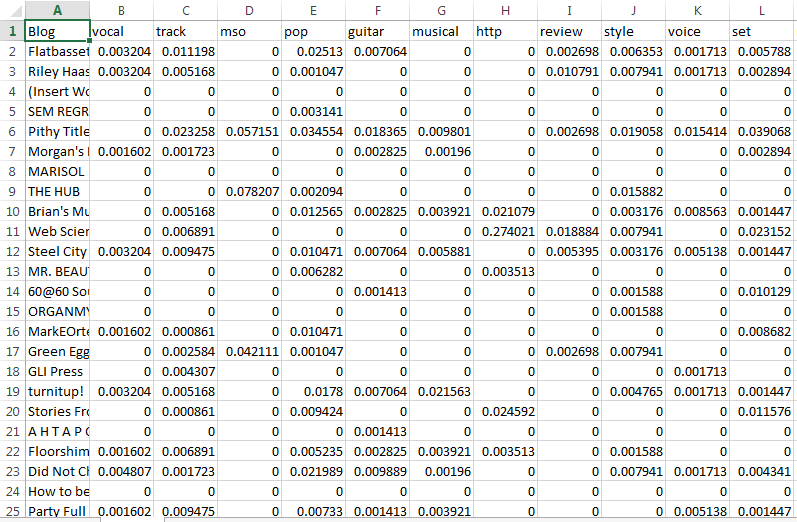
\includegraphics[scale=0.4]{../../q3/output.png}
\centering
\caption{Memento difference}
\label{fig:Initial graph}
\end{figure}
\newpage


\section{Question 4: }
4.  Repeat A3, Q1.  Compare the resulting text from February to 
the text you have now.  Do all 1000 URIs still return a "200 OK" 
as their final response (i.e., at the end of possible redirects)?

Create two graphs similar to that described in Q3, except this 
time the y-axis corresponds to difference in bytes (and not difference
in TimeMap magnitudes).  For the first graph, use the difference
in the raw (unprocessed) results.  For the second graph, use the 
difference in the processed (as per A3, Q1) results.

Of the URIs that still terminate in a "200 OK" response, pick the
top 3 most changed (processed) pairs of pages and use the Unix
"diff" command to explore the differences in the version pairs.

\subsection{Approach}
\begin{itemize}
\item I have extracted raw and processed URIs again which returns status 200.
\item I have found the size of old raw data, new raw data, old processed data, new processed data using size.py.
\item I have found the difference in sizes of old raw data and new raw data and generated a graph.
\item Similarly, I have found the difference in sizes of old processed data and new processed data and generated a graph .
\item I wrote a program statuscode.py to find the status of the existing URIs.
\item I have found that only 784 out of entire 1000 URIs had exited with status code 200.
\item I had found the top three maximum distances of the old and new processed URIs using vim -d command.
\item The  comparision is shown in three seperate screenshots



\end{itemize}
\subsection{Code Listing}
\subsubsection{For extracting raw and processed URIs (extract.py)}
\lstinputlisting[breaklines=True,language=Python]{../../q4/extract.py}
\subsubsection{To find the size of the size of either raw or processed files(size.py)}
\lstinputlisting[breaklines=True,language=Python]{../../q4/size.py}
\subsubsection{To find the number of URIs exiting with status 200 (statuscode.py)}
\lstinputlisting[breaklines=True,language=Python]{../../q4/statuscode.py}
\subsubsection{Generating graph}
\lstinputlisting[breaklines=True,language=Python]{../../q4/Rcommands.R}
\subsection{Output}

\begin{figure}[ht]
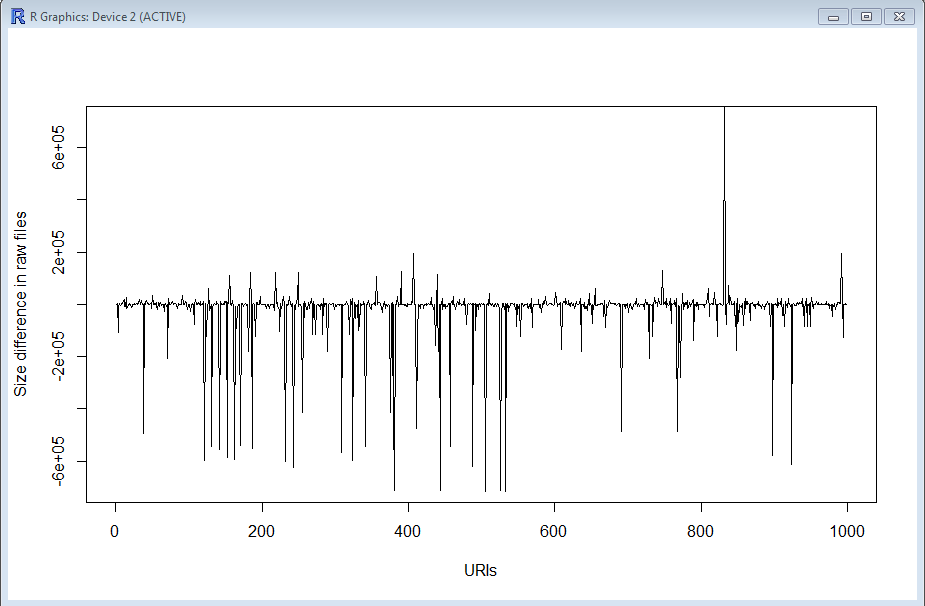
\includegraphics[scale=0.7]{../../q4/rawoutput.png}
\centering
\caption{Raw Difference}
\label{fig:Initial graph}
\end{figure}
\newpage
\begin{figure}[ht]
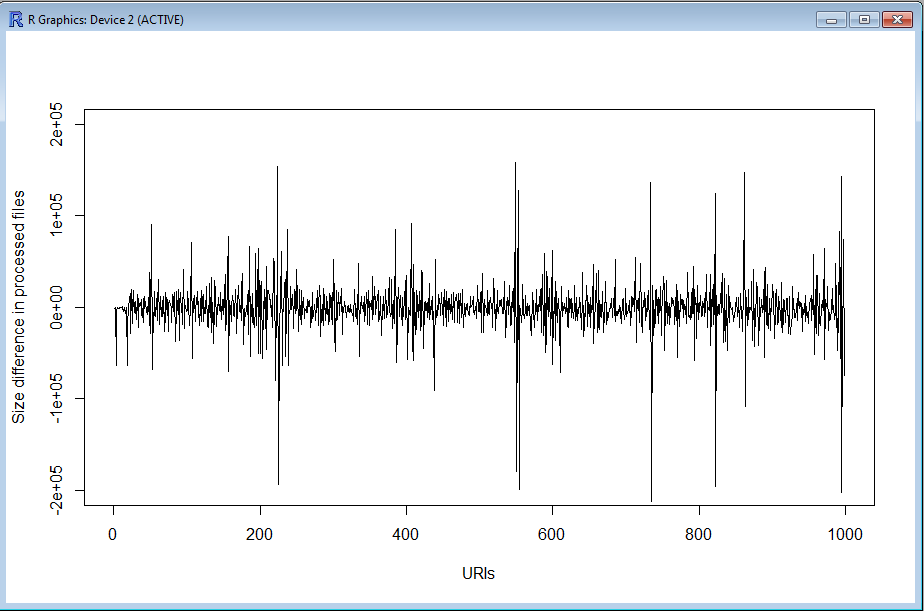
\includegraphics[scale=0.7]{../../q4/processedoutput.png}
\centering
\caption{Processed Difference}
\label{fig:Initial graph}
\end{figure}
\newpage
\begin{figure}[ht]
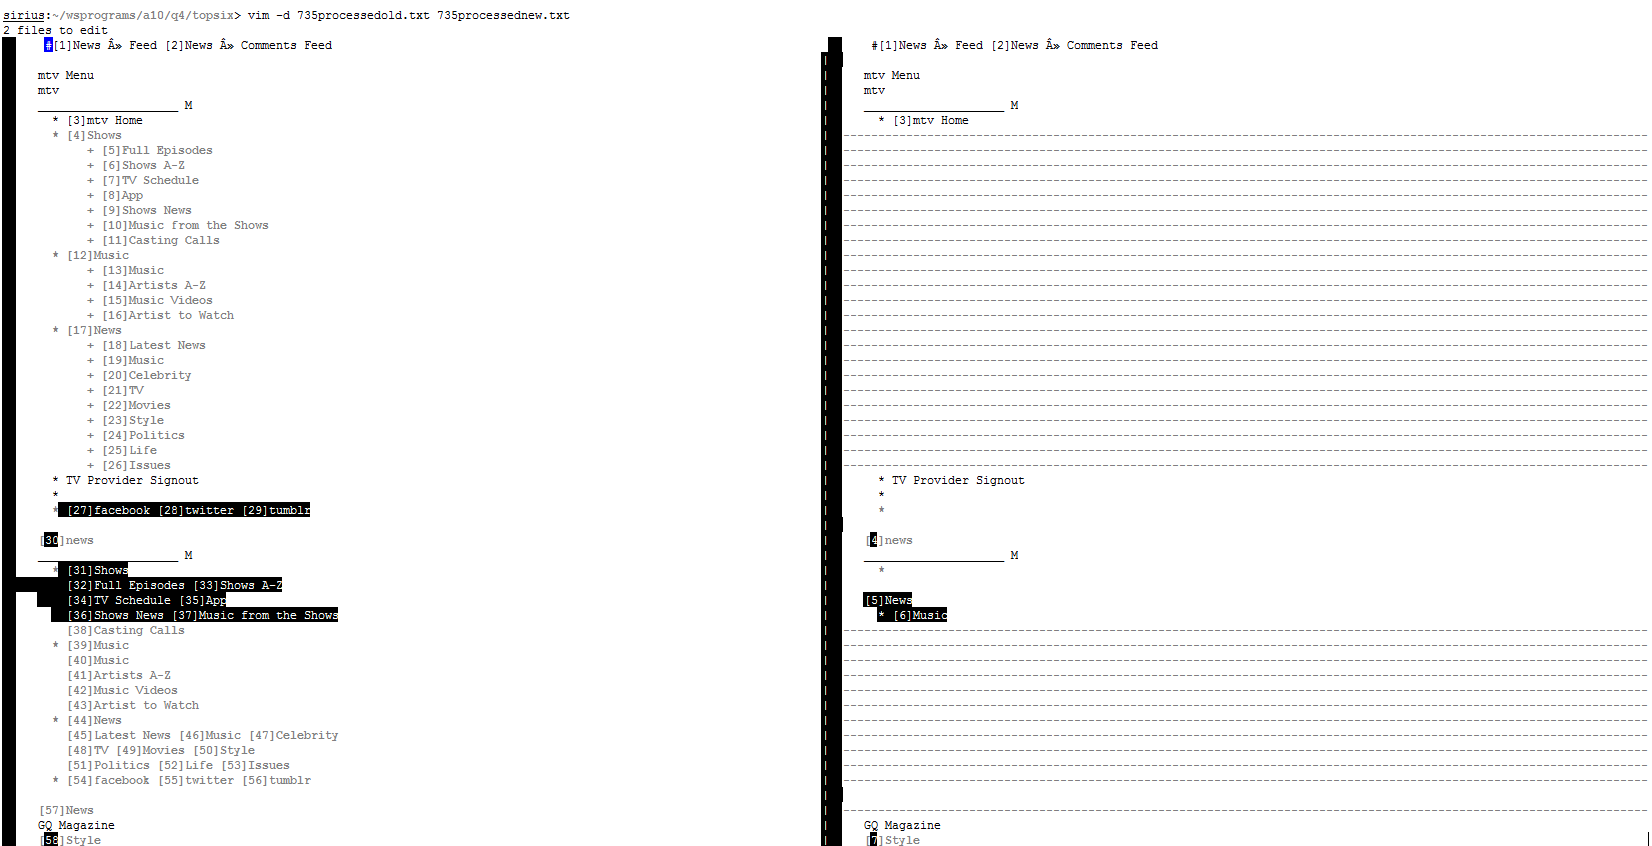
\includegraphics[scale=0.5]{../../q4/735oldvsnew.png}
\centering
\caption{Comparing Processed data of maximum size difference}
\label{fig:Initial graph}
\end{figure}
\newpage
\begin{figure}[ht]
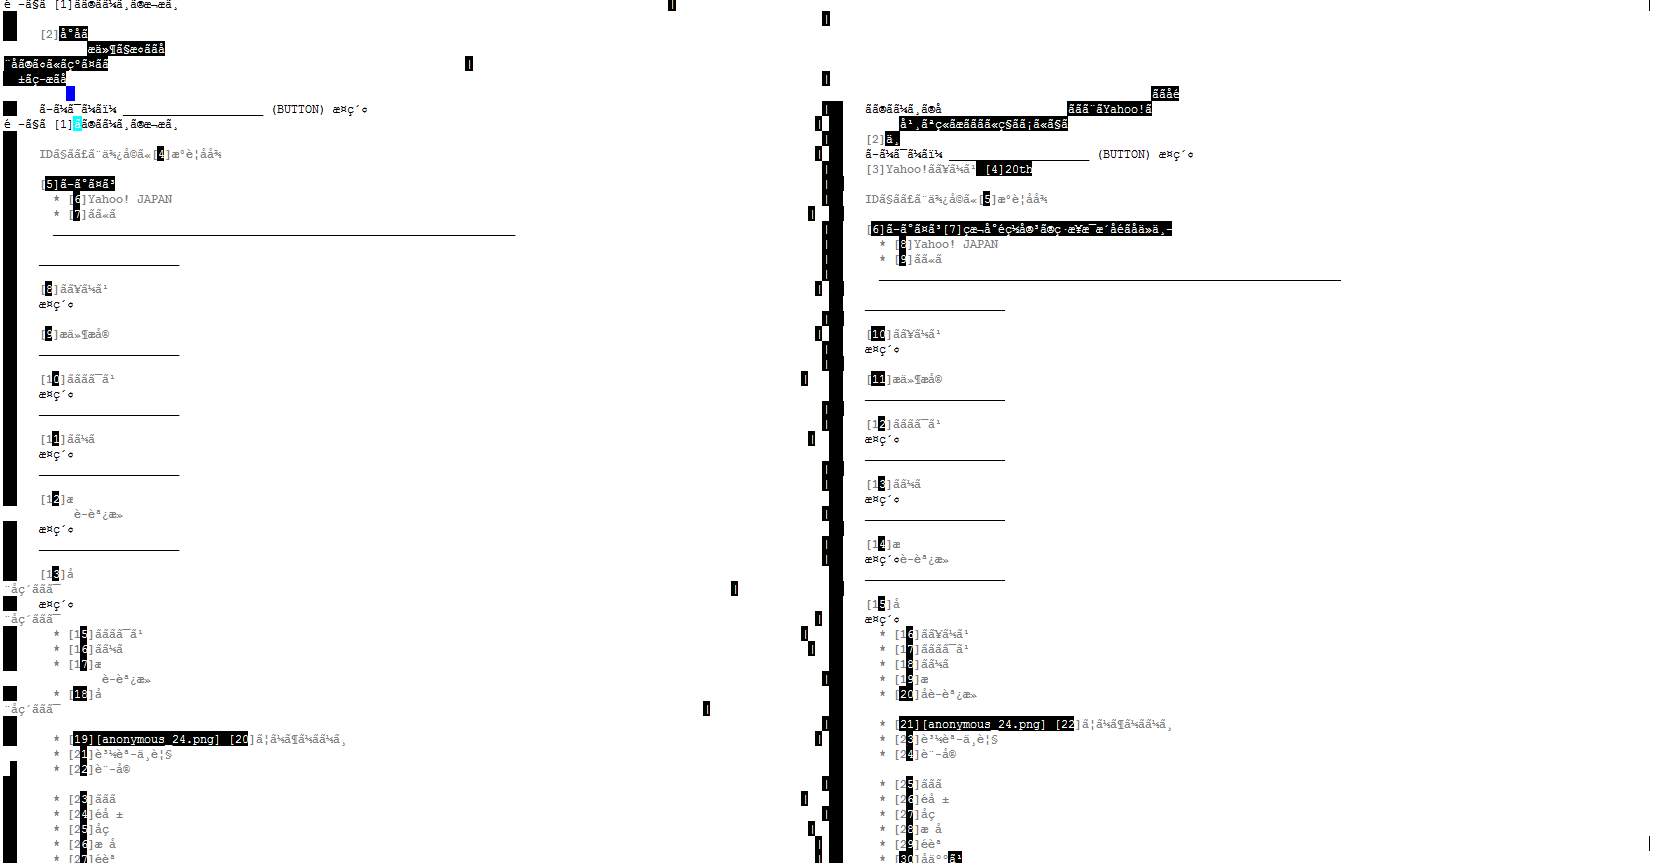
\includegraphics[scale=0.5]{../../q4/995oldvsnew.png}
\centering
\caption{Comparing Processed data of second maximum size difference}
\label{fig:Initial graph}
\end{figure}
\newpage
\begin{figure}[ht]
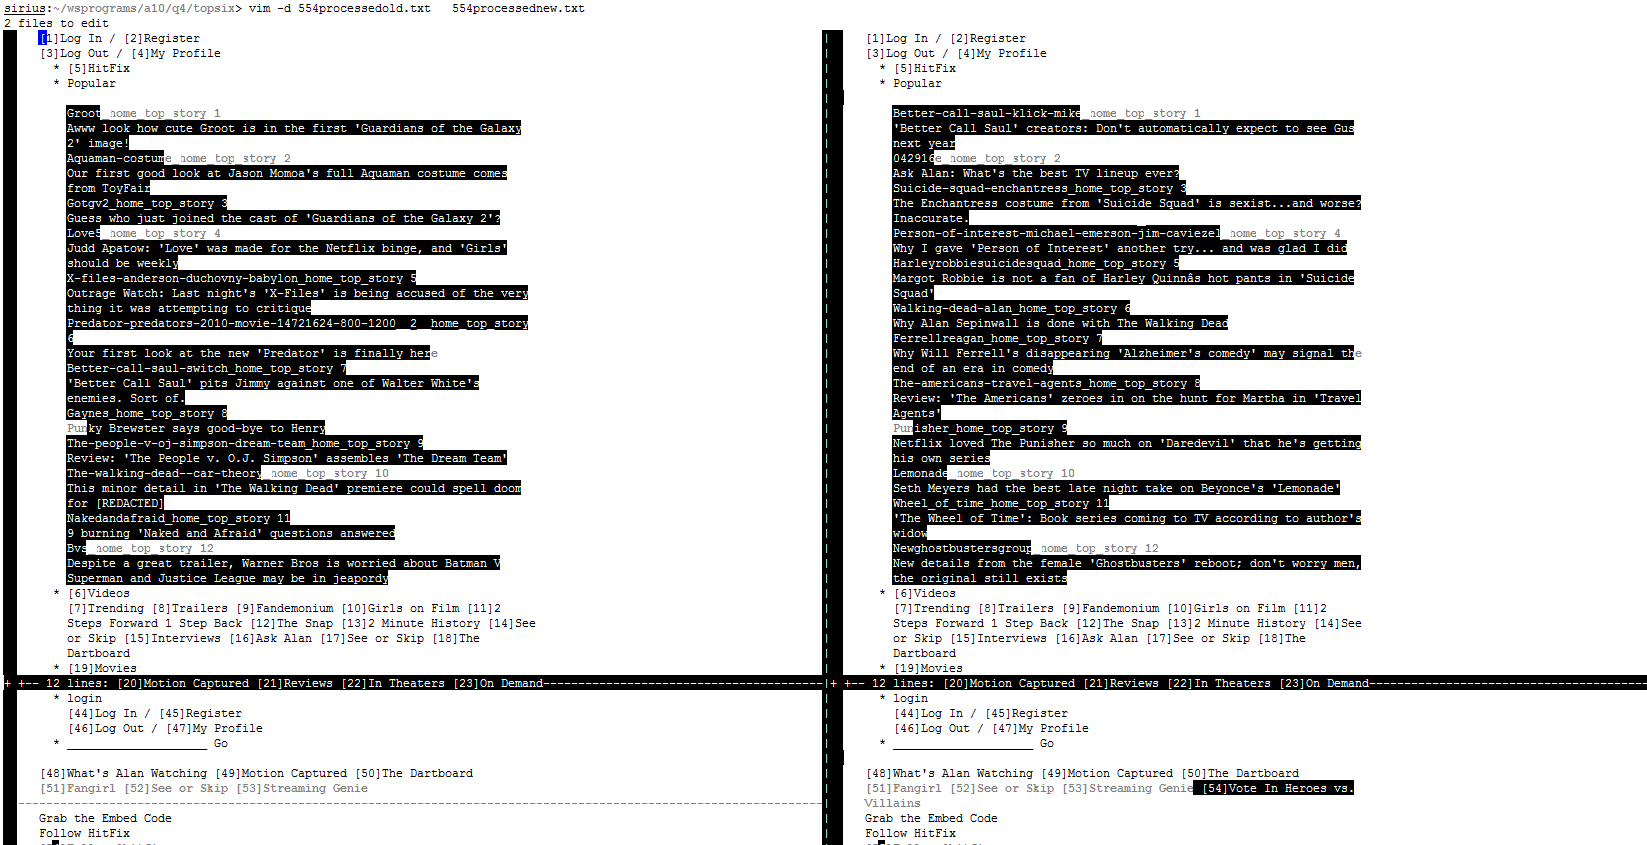
\includegraphics[scale=0.5]{../../q4/554oldvsnew.png}
\centering
\caption{Comparing Processed data of second maximum size difference}
\label{fig:Initial graph}
\end{figure}

\newpage
\addcontentsline{tableofcontents}{section}{References}






\newpage





\bibliographystyle{plain}
\bibliography{references}
\cite{*}
\end{document}